\documentclass{article}

\usepackage{coursenotes}

\set{AuthorName}{TC Fraser}
\set{Email}{tcfraser@tcfraser.com}
\set{Website}{www.tcfraser.com}
\set{ClassName}{General Relativity}
\set{School}{University of Waterloo}
\set{CourseCode}{Phys 476}
\set{InstructorName}{Florian Girelli}
\set{Term}{Winter 2016}

\begin{document}

\titlePage

\tableOfContents

\disclaimer


\section{Introduction}

\subsection{History}

The first lecture was a summary of astrophsyical history from around $\sim$200BC to today. I elected not to take notes as it was pretty standard stuff and a lot of slides. Sorry.

\section{Tensor Formalism}

At the core of General Relativity is the mathematics of differential geometry. Differential geometry requires the idea of tensors, a generalization of vectors and matricies and forms that can handle messy geometries and metrics. \\

Let $V$ be a vector space of finite dimension. Any $V$ is isomorphic to $\R^{n+1}$ through the coefficients of a chosen basis. Let the basis of $V$ be given by,

\[ \bc{e_i}_{i=\tok0n} \]

Then any vector $v \in V$ is expressible by,

\[ v = \sum_{i=0}^{n} v^i e_i \]

Where $v^i$ are the $i$-th coefficients of the vector $v$ with respect to the basis $\bc{e_i}$.

\subsection{Einstein Summation Rule}

For convenience let's provide a new, shorter notation for the vector $v$.

\[ v^ie_i = v^0e_0 + \ldots + v^ne_n = \sum_{i=0}^nv^ie_i \]

Effectively, we have just \textbf{dropped the summation sign}. The einstein summation rule is as follows: \\

If there are two identical indices, 1 ``up'' and 1 ``down'', it means that a summation is secretly present, it's just be removed for convenience. Note that the $i$ in this case is \textit{dummy index}.

\[ v^ie_i = v^{\alpha}e_{\alpha} = v^je_j \]

Here $v^i$ are the components of vector $v \in V$ and are real numbers. $v^i \in \R, \forall i \in \bc{\tok0n}$. \\

Note $v^i$ is called the vector $v$ when $i$ is the set $\bc{\tok0n}$, but can also be called the $i$-th component of $v$ when $i$ has a fixed value $i \in \bc{\tok0n}$. \\

\subsection{Examples of Basis for V}

The values of $e_i$ or the $i$'s themselves can take on many possible values.

\begin{itemize}
    \item Cartesian coordinates $t,x,y,z$
    \item spherical coordinates $t, r, \phi, \theta$
    \item etc.
\end{itemize}

Each of the above examples is the space $V = \R^4$ (with some bounds for spherical coordinates).

\subsection{Dual Vector Space}

The dual vector space of $V$ denoted $V^*$ is also isomorphic to $\R^{n+1}$ and is built from the space of linear forms on V.

\[ V^* = \bc{w: V \ar \R \st w(\alpha v_1 + \beta v_2) = \alpha w( v_1) + \beta w(v_2)} \]

where $v_1, v_2 \in V$ and $\alpha, \beta \in \R$.

In Quantum Mechanics, the vectors are the bras and the elements of the dual space (called the co-vectors) are the kets. \\

We note,

\[ \bc{f^i}_{i=\tok0n} \]

is the basis for $V^*$ is defined by the kronecker symbol $\delta$,

\[ f^j(e_j) = {\delta^j}_i \]

\[ {\delta^j}_i = \piecewise{1}{i=j}{0}{i\neq j} \]

An element in $V^*$ is $w = w_if^i$. $w_i$ are the components of the covector $w$. Note that for a \textbf{finite dimensional vector space},

\[ V^{**} = V \]

\subsection{Bilinear Maps}

Introduce a bilinear map $B(v, w)$ where $B: V \cross V \ar \R$ where,

\[ B(\alpha v_1 + \beta v_2, w) = \alpha B(v_1, w) + \beta B(v_2, w) \]

and the same for the other parameter $w$. \\

Examples include the inner product (otherwise known as the scale or dot product).

Bilinear forms are bilinear maps such that the following conditions are true:

\begin{itemize}
    \item symmetric: $B(v,w) = B(w,v)$
    \item non-degenerated: $B(v,w) = 0 \quad \forall v \implies w = 0$
\end{itemize}

Playing with indices,

\begin{align*}
    B(v,w) &= B(v^\alpha e_\alpha, w^\beta e_\beta) \\
           &= v^\alpha B( e_\alpha, w^\beta e_\beta) \note{By linearity} \\
           &= v^\alpha w^\beta B( e_\alpha, e_\beta) \note{By linearity}
\end{align*}

A bilinear map used in this way provides a way to eliminate the headache of complicated cross sums. Define new notation,

\[ B( e_\alpha, e_\beta) \defined g_{\al\be} \]

Where $g_{\al\be}$ is a real number $\R$ because $\al$ and $\be$ are summed over.

\[ B(v, w) = v^\al w^\be g_{\al\be} = v^\al g_{\al\be}w^\be =  w^\be g_{\al\be} v^\al \]

All of the above terms are commutative because in the end, it represents a sum over all $\al, \be$.

\[ B(v,w) = \underbrace{v^0w^0g_{00} + \ldots + v^2w^3g_{2,3} + \ldots + v^nw^ng_{nn}}_{(n+1)^2 \text{terms}} \]

\subsection{Distance and Norms}

To define a distance in a vector space, we can use norms. In this case, $g_{\al\be}$ would be called the metric. The Euclidean metric (with respect to a cartesian basis) for example would be,

\[ g_{\al\be} = \piecewise{1}{\al = \be}{0}{\al \neq \be}  \]

We can also choose to enforce that the basis be orthonormal,

\[ B(e_i, e_j) = \piecewise{\pm1}{i = j}{0}{i \neq j} \]

Note that the potential for a negative norm means the notion of positive definiteness is no longer gauranteed.

\subsection{Signatures of Metrics}

We call the signature of the metric the number of $+1$'s and $-1$'s appearing in $g_{ij}$ when dealing with the orthonormal basis. Signature is denoted as:

\[ \br{p, q} = \br{\underbrace{p}_{\text{postive}}, \underbrace{q}_{\text{negative}}} \]

For example,

\begin{itemize}
    \item Euclidean metric: $(n+1, 0)$
    \item Minkowski metric: $(n, 1)$
\end{itemize}

Note the order of the signature is chosen to be $(p,q)$ and not $(q, p)$ by convention.

\subsection{Co-vectors from Vectors}

Note that $v^i$ was called the vector and $w_i$ was called the covector. This notation seems to indicate that conversion between $V$ and $V^*$ is notationally equivalent to raising and lowering the indices. \\

We call the following opperation ``Lowering the index using the metric''.

\[ \underbrace{v^\al}_{\text{components of vector}} \mapsto g_{\al\be} v^\be = \underbrace{v_\al}_{\text{components of covector}} \]

In use,

\[ B(v,w) = v^\al g_{\al\be} w^\be = \untext{v_\be}{bra} \untext{w^\be}{ket} \]

\subsection{Linear Map on V to V}

\[ M : V \ar V \]

Where M is a matrix. An the map is equivalent to $v \ar Mv \in V$. Some definition,

\[ \br{Mv}^\al = \untext{{M^\al}_\be}{Matrix \\ (components)} v^\be \]

Note that ${M^\al}_\be \in \R$ for $\al$ and $\be$ fixed. Example: The identity matrix is denoted ${\delta^\al}_\be = \mathbb{I}$.

\subsection{Scalar Product on Dual Space}

Introduce a scalar product for the co-vectors $w$.

\[ w, t \in V^* \]

\[ w \cdot t = w_\al h^{\al\be} t_\be \]

Where $h^{\al\be}$ is symmetric and non-degenerate.

So how is the scalar product between the dual and normal space related? Specifically how are $g_{\al\be}$ and $h^{\al\be}$ connected? Well,

\begin{align*}
   v^\al g_{\al\be} w^\be &= v^\al w_\al \\
   &= v_\ga h^{\ga\al} w_\al \\
   &= v^\nu g_{\nu\ga} h^{\ga\al} w_\al \\
   &= v^\nu g_{\nu\ga} h^{\ga\al} g_{\al\mu} w^\mu
\end{align*}

Since this is true for any $v$ and $w$ we require that,

\[ h^{\ga\al} g_{\al\mu} = {\delta^\ga}_\mu \]

This means we say that the metric $h$ is the inverse of the metric $g$. Convention on $V^*$: we denote the metric $g^{\al\be}$ (the indices are ``up''). \\

\subsection{Invariance of Scalar Product}

Let us say we have a matrix $M : v \ar \ti{v} = Mv, w \ar \ti{w} = Mw$ and that $M$ preserves the scalar product.

\[ \ti{v} \cdot \ti{w} = v \cdot w \qquad \forall v, w \]

Examine,

\[ {M^\ga}_\al v^\al g_{\al\be} {M^\be}_\rho w^\rho = v^\al g_{\al\be}w^\be \]

Use communitivity and dummyness of indices to obtain,

\[ v^\al {M^\ga}_\al g_{\al\rho} {M^\rho}_\be w^\be = v^\al g_{\al\be}w^\be \]

Drop outer co-vectors $v$ and $w$ to get,

\[ {M^\ga}_\al g_{\al\rho} {M^\rho}_\be = g_{\al\be} \numberthis \label{eq:invarM} \]

Note that this expression is consistent with the Einstein summation convention. \\

An example of an $M$ on euclidean space could be a rotation matrix, or the identity. \\

When $M$ satisfies \ref{eq:invarM}, it is said to be orthogonal. It $\det(M) = 1$ then we say that $M$ is \textit{special}.

\subsection{Trace of M}

What is the trace of $M$?

\[ \Tr(M) = {M^\al}_\al = {M^0}_0 + \ldots + {M^n}_n\]

This is just a notationally convention. It is the sum of the diagonal terms of $M$.

\subsection{Tensor Product}

A tensor product makes a linear map a multi-linear map.

\heading{Theorem}

Let $E$ and $F$ be 2 vector spaces (with finite dimensionality.)

$\exists $ a unique ($!$) set (up to isomorphism) $E \otimes F$ such that if $f$ is a bilinear map $f: E \cross F \ar \R$ then $\exists$ a linear map $f^* : E \otimes F \ar \R$ such that $f = f^* \circ \phi$ with

\begin{center}
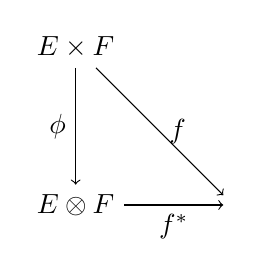
\begin{tikzpicture}
\node (EtimesF) at (0,0) {$E \times F$};
\node (EotimesF) at (0,-2) {$E \otimes F$};
\node (R) at (2,-2) {$\R$};
\draw [->] (EtimesF) edge node[left] {$\phi$} (EotimesF);
\draw [->] (EtimesF) edge node[right] {$f$} (R);
\draw [->] (EotimesF) edge node[below] {$f^*$} (R);
\end{tikzpicture}
\end{center}

Then we have,

\[ \Lin(E \otimes F, \R) \iso \Bin(E \cross F, \R) \]
\[ \Lin(f^*, \R) \iso \Bin(f, \R) \]

where `$\iso$' is used to denote \textit{isomorphic}.

\heading{Properties}

Basis for $E \otimes F$ is $e_\al \otimes g_\al$ where $e_\al$ is the basis for E and $g_\al$ is the basis for F.
For $a \in \R$ and $t, v \in E$, $u, w \in F$,

\begin{itemize}
    \item $\dim(E \otimes F) = \dim(E)\dim(F)$
    \item $a (v \otimes w) = (av) \otimes w = v \otimes (aw)$
    \item $(v + t) \otimes w = v \otimes w + t \otimes w$
    \item $v \otimes (w + u) = v \otimes w + v \otimes u$
    \item $a \otimes w = aw$
    \item $\R \otimes F = F$
\end{itemize}

Note that $V^* \otimes V^* \iso \Bin(V \times V, \R)$. To motivate this, let $f^\al \otimes f^\be$ be the basis for $V^* \otimes V^*$, and then a general element in $V^* \otimes V^*$ is,

\[ t = t_{\al\be} f^\al \otimes f^\be \]

Note that $t_{\al\be}$ is just a set of numbers. Then the tensor product is expanded as follows,

\begin{align*}
    t (v \otimes w) &= t (v^\al e_\al \otimes w^\be e_\be) \\
    &= t_{\ga\de} (f^\ga \otimes f^\de) (v^\al e_\al \otimes w^\be e_\be) \\
    &= t_{\ga\de} v^\al w^\be (f^\ga \otimes f^\de) (e_\al \otimes e_\be) \note{By linearity} \\
    &= t_{\ga\de} v^\al w^\be f^\ga(e_\al) f^\de(e_\be) \note{By foiling and definition of $f$} \\
    &= t_{\ga\de} v^\al w^\be {\delta^\ga}\al {\delta^\de}_\be \\
    &= t_{\ga\de} v^\ga w^\be {\delta^\de}_\be \note{By sifting property of $\delta$}\\
    &= t_{\ga\de} v^\ga w^\de \note{By sifting property of $\delta$ again}
\end{align*}

Since $t (v \otimes w)$ is the tensor product $V^* \otimes V^*$ and $t_{\ga\de}$ is the components of the bilinear form, one can see the connection $V^* \otimes V^* \iso \Bin(V \times V, \R)$. \\

Tensors allow one to write bilinear maps as linear maps. What about multi-linear maps?

\heading{Tensors}

A tensor of rank $\br{k,l}$ is a multilinear map

\[ \underbrace{V^* \times \cdots \times V^*}_{k} \times \underbrace{V \times \cdots \times V}_{l} \ar \R \]

which transforms \textit{well} under the change of basis of $V$ and $V^*$. \\

\begin{center}
\label{Tensor Examples}
\begin{tabular}{c|c}
Tensor & Rank \\
\hline
vectors & $(1,0)$ \\
co-vectors & $(0,1)$ \\
scalar & $(0,0)$ \\
metric & $(0,2)$ \\
inverse metric & $(2,0)$ \\
matrix & $(1,1)$ \\
\end{tabular}
\end{center}

The set of tensors of rank $(k,l)$ is a vector space of dimension $n^{k+l}$ (if $V$ has dimension $n$). Checking with the examples above motivates this fact. \\

Using the basis $e_{\al_1} \otimes \cdots \otimes e_{\al_k} \otimes f^{\be_1} \otimes \cdots \otimes f^{\be_k}$

\[ T = {T^{\al_1\al_2\cdots\al_k}}_{\be_1\be_2\cdots\be_l} e_{\al_1} \otimes \cdots \otimes e_{\al_k} \otimes f^{\be_1} \otimes \cdots \otimes f^{\be_k}\]

For fixed $\al_i$ and $\be_i$ this is a real number in $\R$. These are the \textit{components of the tensor}. \\

By abuse of notation we will call ${T^{\al_1\al_2\cdots\al_k}}_{\be_1\be_2\cdots\be_l}$ the tensor. \\

We are talking about these transformations as change of basis of $V$ and $V^*$. Examples:
\begin{itemize}
  \item rotations (boost)
  \item change of coordinates from Cartesian to spherical, cylindrical, etc.
\end{itemize}

We can have a linear change of basis $\ti{x}^\mu = {A^\mu}_\nu x^\nu $.

\heading{Example}

\begin{center}
\begin{tabular}{c|c}
    Cartesian & Polar \\
    \hline
    $e_1 = \vec{i}$ & $\ti{e}_1 = e_r$ \\
    $e_2 = \vec{j}$ & $\ti{e}_2 = e_\theta$ \\
\end{tabular}
\end{center}

\heading{Example}

\[ \ti{e}_\al = \untext{\pder{x^\nu}{\ti{x}^\al}}{Jacobian} e_\nu = {A^{\nu}}_\al e_\nu \]

Note: \textit{Up in the denominator means down on the original coordinates (LHS).}

For example,

\begin{center}
\begin{tabular}{c|c}
    $x^1 = x$ & $\ti{x}^1 = r$ \\
    $x^2 = y$ & $\ti{x}^2 = \theta$ \\
\end{tabular}
\end{center}

\[ \ti{e}_1 = e_r = \pder{x^1}{\ti{x}^1} e_1 + \pder{x^2}{\ti{x}^1} e_2 = \cos \theta e_1 + \sin \theta e_1 \]
\[ \ti{e}_2 = e_\theta = \pder{x^1}{\ti{x}^2} e_1 + \pder{x^2}{\ti{x}^2} e_2 = - r \sin \theta e_1 + r \cos \theta e_1 \]

\heading{Vectors in multiple basis}

\[ v = v^\nu e_\nu = \ti{v}^\nu \ti{e}_\nu \]

With conversion of basis given by,

\[ \ti{e}_\al = {A^\nu}_\al e_\nu\]

Thus substituting in,

\[ v^\nu e_\nu = \ti{v}^\al {A^\nu}_\al e_\nu \note{Drop $e_\nu$}\]

\[ v^\nu = \ti{v}^\al {A^\nu}_\al \]

But with $A$ as a Jacobian,

\[ v^\nu = \pder{x^\nu}{\ti{x}^\al} \ti{v}^\al \]
\[  \ti{v}^\al = \pder{\ti{x}^\al}{x^\nu} v^\nu \]

But what about the dual space?

By definition,

\[ \ti{f}^\be\br{\ti{e}_\nu} = \delta^\be_\mu = \ti{f}^\be \br{{A^\al}_\nu e_\al} = {A^\al}_\nu \ti{f}^\be \br{ e_\al}\]

Let $\ti{f}^\be \br{ e_\al}$ be expressed as $\ti{f}^\be = {B^\be}_\ga f^\ga$

\begin{align*}
    \ti{f}^\be\br{\ti{e}_\nu} &= {A^\al}_\nu {B^\be}_\ga f^\ga \br{ e_\al} \\
    &= {A^\al}_\nu {B^\be}_\ga {\delta^\ga}_\al \\
    &= {B^\be}_\ga {A^\ga}_\nu \\
    &= {\delta^\be}_\nu
\end{align*}

Thus $B$ is the inverse of $A$. \\

What does transforming \textit{well} mean? A tensor is transforming well if its components transform as

\[{T^{\nu_1\nu_2\cdots\nu_k}}_{\al_1\al_2\cdots\al_l} \ar \pder{\ti{x}^\nu_1}{x^\be_1} \cdots \pder{\ti{x}^\nu_k}{x^\be_k} \pder{x^\ga_1}{\ti{x}^\al_1} \cdots \pder{x^\ga_k}{\ti{x}^\al_k} {T^{\be_1\be_2\cdots\be_k}}_{\ga_1\ga_2\cdots\ga_l} = {\ti{T}^{\nu_1\nu_2\cdots\nu_k}}_{\al_1\al_2\cdots\al_l} \]

If you find something like ${T^\al}_\be$, is it a tensor? \textbf{No! You must check if it transforms well.}

\[ \pder{}{x^\nu} v^\al \note{This is not a tensor.} \]

The derivative here prevents it from being well-formed. In the future we will define a derivative that allows a tensor to transform well.

\subsection{Operations on Tensors}

\begin{itemize}
    \item Add (with matching rank): ${T^{\al_1\al_2}}_{\be_1\be_2} + {C^{\al_1\al_2}}_{\be_1\be_2}$.
    \item Contraction (partial trace): $\mathcal{T} (k, k) \ar \mathcal{T} (k-1, k-1)$.
    \begin{itemize}
        \item ${T^{\al_1\cdots\al_i\cdots\al_k}}_{\be_1\cdots\be_j\cdots\be_l} \ar {T^{\al_1\cdots\al_i\cdots\al_k}}_{\be_1\cdots\al_j\cdots\be_l}$
    \end{itemize}
    \item ``Outer'' Product (Gluing together tensors)
    \begin{itemize}
        \item $\mathcal{T}(k,l) \times \mathcal{T}(k',l') \ar \mathcal{T}(k + k', l+ l')$
        \item $(T_1, T_2) \ar T_1T_2$
        \item $T_1 T_2 \ar {T_1^{\nu_1\cdots\nu_k}}_{\al_1\cdots\al_l} {T_2^{\be_1\cdots\be_k}}_{\ga_1\cdots\ga_l}$
        \item \textbf{Example:} $\br{v^\al, w_\be} \ar v^\al \otimes w_\be = v^\al w_\be$. (In QM this is $\ket{\phi}\bra{\varphi}$)
    \end{itemize}
\end{itemize}

The metric $g_{\al\be}$ can change the rank of a tensor. Recall a metric is rank $(0,2)$ is symmetric and is non-degenerate.

\heading{Example}

Changing from rank $(1,0)$ to rank $(0,1)$:

\[ v^\al \ar v_a = g_{\al\be} v^\be \]

Changing from rank $(2,2)$ to rank $(4,0)$:

\[ {C^{\al\be}}_{\ga\de} \ar C_{\al\be\ga\de} = g_{\al\rho}g_{\be\eta} {C^{\rho\eta}}_{\ga\de} \]

Changing from rank $(2,2)$ to a different rank $(2,2)$:

\[ {C^{\al\be}}_{\ga\de} \ar {{{C^{\al}}_\be}^{\ga}}_\de = g_{\be\rho}g^{\ga\eta} {C^{\al\rho}}_{\eta\de} \]

\subsection{Facts About Tensors}

\heading{Order Matters}

The order of indices that label a tensor is \textbf{very} important. It indicates the product space you are mapping \textit{from} to $\R$.
\begin{align*}
{C^\al}_\be &: \qquad V^* \times V \ar \R \\
{C_\al}^\be &: \qquad V \times V^* \ar \R \\
C_\al^\be &: \qquad \text{Nothing. Don't do this.} \\
\end{align*}

\heading{Equality between tensors}

As tensors, indices must match:\\

Position of indices is matching: ${{C^\al}_\ga}^\de = {{T^\al}_\ga}^\de$ \\

Position of indices is \textbf{not} matching: ${{C^\al}_\ga}^\de \neq {{T^\al}_\ga}_\de$ \\

But for fixed $\al, \ga, \de$, one can abuse the notation a bit:

\[ {{C^\al}_\ga}^\de = {{T^\al}_\ga}_\de \note{Try to avoid this.}\]

\subsection{Outer Product and Contraction}

\heading{Example}

Outer Product: ${M^{\al}}_\be{M^{\ga}}_\de = {{{{C^{\al}}_\be}^\ga}_\de}$ \\
Contraction: ${M^{\al}}_\be{M^{\be}}_\de = {{{{C^{\al}}_\be}^\be}_\de} = {C^\al}_\ga$

\heading{Example}

Outer product and contraction: ${C^{\al\be}}_{\ga\de}{T^{\ga\de}}_{\rho} = {A^{\al\be}}_\rho$ \\
This doesn't make sense: ${C^{\al\be}}_{\ga\ga}{T^{\ga\de}}_{\rho} = ??$ \\

Note, when there is a ``+'' sign we can be ``loose'' with the indices. Here the dual indices \textbf{do not} indicate a summation. This acts as an abuse of notation, but is sometimes difficult to avoid.

\[ C^{\al\ga}{T_\ga}^{\de} + {F_\ga}^{\de}A^{\al\ga} \]

\subsection{Interpretation of Tensors}

By looking at the indices, how can we interpret the physical meaning of the tensor object? \\

\begin{tabular}{c|l}
    Tensor & Interpretation \\
    \hline
    $v^\nu$ & vector \\
    $v_\nu$ & covector \\
    ${M^\al}_\be$ & matrix ($\al$ rows, $\be$ columns) \\
    ${M^\al}_\al$ & contracted matrix (trace) \\
    ${M^{\al\ga}}_\de$ & matrix whose elements are vectors themselves (${\cdot^\ga}_\de$ is the matrix) \\
    ${M^{\al\ga}}_\de$ & vector with matrix components (${M^\al}$ is the vector) \\
    ${R^{\al\be}}_{\ga\de}$ & matrix of matricies *\\
\end{tabular}
\vspace{0.1in}

*For example, if $\dim V = 4$, ${R^{\al\be}}_{\ga\de}$ has $4^4 = 256$ components. Note however, there can be many symmetries that reduce the number of unique components.

\subsection{Symmetry of Tensor}

We can always build a symmetric and antisymmetric part of a tensor $T^{\al\be}$. Let's look at the case of 2 indices $\al, \be$:

\heading{Symmetric Part}

\[ T_{\br{\al\be}} = \f12 \br{T_{\al\be} + T_{\be\al}} \]
\[ T_{\br{\al\be}} = T_{\br{\be\al}}  \]

\heading{Antisymmetric Part}

\[ T_{\bs{\al\be}} = \f12 \br{T_{\al\be} - T_{\be\al}} \]
\[ T_{\bs{\al\be}} = - T_{\bs{\be\al}}  \]

Note that for all tensors $T^{\al\be} = T^{\br{\al\be}} + T^{\bs{\al\be}}$. This acts as the decomposition into odd and even symmetries of the tensor. \\

For more indices:

\[ {T^{\br{\al\be}}}_{\bs{\ga\de}} = \f14\br{{T^{\al\be}}_{\ga\de} + {T^{\be\al}}_{\ga\de} - {T^{\al\be}}_{\de\ga} - {T^{\be\al}}_{\de\ga}} \]

What does $T^{\br{\al\be\ga}}$ mean? For that we will need a permutation group.

\section{Physics Review}

Moving away from tensors for a moment... \\

\subsection{Newtonian Physics}

According to Galileo and Newton, we got the interpretation that both space and time is flat $\br{\R^3}$ and is absolute. More specifically, all clocks will have the same time if they are started/synced at some shared moment. It is built on cartesian coordinate system: $\br{\vec{x}, t}$. With this we say that an object is at position $\vec{x}$ at time $t$. In this context, coordinates are \textit{outcomes of measurements}. In General Relativity, the notion of coordinates can be quite different. \\

Consider a particle (2d spacetime):

\begin{center}
\begin{tikzpicture}[scale=1.0]
    % Draw axes
    \draw [<->,thick] (0,4) node (yaxis) [above] {$x$}
        |- (5,0) node (xaxis) [right] {$t$};
    \draw [blue, thick, ->] plot [smooth, tension=1] coordinates { (0,1) (1,2) (3,1) (4,3)};
    \node [blue,above] (label) at (1,2) {$x(t)$};
\end{tikzpicture}
\end{center}

Typically, $x$ is drawn as the ordinate ($y$-axis) and $t$ as the abscissa ($x$-axis).

\heading{Spacetime diagram}

In a spacetime diagram, $t$ is drawn as the ordinate.

\begin{center}
\begin{tikzpicture}[scale=1.0]
    % Draw axes
    \draw [<->,thick] (0,4) node (yaxis) [above] {$t$}
        |- (5,0) node (xaxis) [right] {$x$};
    \draw [blue, thick, ->] plot [smooth, tension=1] coordinates { (1,0) (2,1) (1,3) (3,4)};
    \node [blue, right] (label) at (2,1) {$x(t)$};
\end{tikzpicture}
\end{center}

If we begin to use light to probe the position of objects, we are going to run into some surprising results. We will have to abandon Newtonian Physics and switch to the domain of Special Relativity.

\subsubsection{Newton's Dynamical Law \& Inertial Observers}

\[ \vec{F} = m \vec{a}\]

Where $\vec{F}$ is the total force applied to the system, $\vec{a} = \ddot{\vec{x}} = \dder{\vec{x}}{t}$ and $m$ is the inertial mass. For $\vec{x}$ is it convienent to use the Cartesian coordinate system. \\

If $\vec{F} = \vec{0}$ then the dynamics becomes $\ddot{\vec{x}} = 0$ which yields solution,

\[ \vec{x}(t) = \vec{v} t + \vec{x}_0 \]

Where $\vec{x}_0$ is the initial condition and $\vec{v}$ is the velocity in the observer's frame. This solution describes a straight line.

\begin{center}
\begin{tikzpicture}[scale=1.0]
    % Draw axes
    \draw [<->,thick] (0,4) node (yaxis) [above] {$\vec{x}$}
        |- (5,0) node (xaxis) [right] {$t$};
    \draw [blue, thick, ->] plot [smooth, tension=1] coordinates { (1,0) (3,4)};
    \node [blue, right] (label) at (2,1) {$\vec{x}(t) = \vec{v}t + \vec{x}_0$};
\end{tikzpicture}
\end{center}

However, consider this solution in a spacetime diagram,

\begin{center}
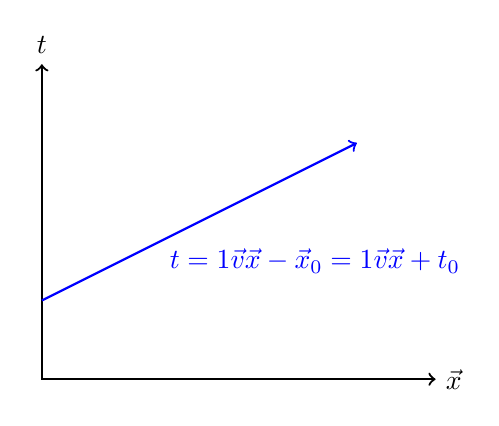
\begin{tikzpicture}[scale=1.0]
    % Draw axes
    \draw [<->,thick] (0,4) node (yaxis) [above] {$t$}
        |- (5,0) node (xaxis) [right] {$\vec{x}$};
    \draw [blue, thick, ->] plot [smooth, tension=1] coordinates { (0,1) (4,3)};
    \node [blue, right] (label) at (1.5,1.5) {$t = \f{1}{\vec{v}}\br{\vec{x} - \vec{x}_0} = \f{1}{\vec{v}}\vec{x} + t_0$};
\end{tikzpicture}
\end{center}

\heading{Definition}

The class of frames (observers) for which the the dynamics of a system is $\ddot{\vec{x}} = \vec{0}$ are called an inertial observers.

\begin{center}
\begin{tikzpicture}[scale=1.0]
    % Draw axes
    \coordinate (nya) at (0, -1);
    \coordinate (pya) at (0, 3);
    \coordinate (nxa) at (-2, 0);
    \coordinate (pxa) at (4, 0);
    \draw [<->, thick] (nya) -- (pya);
    \draw [<->, thick] (nxa) -- (pxa);
    \node [above] (lpya) at (pya) {$t$};
    \node [right] (lpxa) at (pxa) {$x$};
    \draw [orange, thick, ->] plot [smooth, tension=1] coordinates {(nya) (pya)};
    \node [orange] (label) at (-0.5, 0.5) {$x(t)$};
    \draw [red, thick, ->] plot [smooth, tension=1] coordinates {($(nya) + (1,0)$) ($(pya) + (1,0)$)};
    \node [red] (yellowlabel) at (2, 0.5) {translation};
    \draw [blue, thick, ->] plot [smooth, tension=1] coordinates {(-0.5, -1) (1.5, 3.0)};
    \node [blue, right] (label) at (1.5, 3.0) {boost};
\end{tikzpicture}
\end{center}

Note that rotations are not visible in this diagram as there is only one 1 space dimension.

Transformations that relate inertial observers:
\begin{itemize}
    \item translation: $\vec{x}(t) \ar \vec{x}'(t) = \vec{x}(t) + \vec{a}$
    \item rotation: $\vec{x}(t) \ar \vec{x}'(t) = R \cdot \vec{x}$
    \item Galilean boost: $\vec{x}(t) \ar \vec{x}'(t) = - \vec{v}t  + \vec{x}(t)$
\end{itemize}

For each of these transformations $\ddvec{x}' = \vec{0}$. We will now prove the set of all these transformation of $\vec{x}(t) \ar \vec{x}'(t)$ form a group.

\heading{Groups}

A Group is a set $G$ equipped with an associated product ($\cdot$), a unit element and an inverse.

\begin{itemize}
    \item $g_1 \cdot g_2 = g \in G, g_i \in G$
    \item $g_1 \cdot \br{g_2 \cdot g_3} = \br{g_1 \cdot g_2} \cdot g_3$
    \item $g \cdot 1 = 1 \cdot g = g$
    \item $g \cdot g^{-1} = g^{-1} \cdot g = 1$
    \item In general, $g_1 \cdot g_2 \neq g_2 \cdot g_1$.
    \item An abelian group is one where $g_1 \cdot g_2 = g_2 \cdot g_1$.
\end{itemize}

Upon careful examinations of translations and rotation of space $\R^n$, both translations and rotations form a group. What about Galilean boosts? \\

\newcommand{\wrt}{with respect to }

Consider person $A$ (Alice) standing on the ground and person $B$ (Bob) in a rocket traveling with velocity $\vec{v}_1$ \wrt $B$. Give person $B$ a ball in the rocket and let him/her kick it with velocity $\vec{v}_2$ \wrt $B$. What is the velocity of the ball \wrt person $A$? Switching between the perspectives of the system is equivalent to performing a Galilean Boost. \\

\heading{Matrix Representation of a Group}

\begin{center}
\begin{tikzpicture}[scale=1.0]
    % Draw axes
    \coordinate (nya) at (0, -1);
    \coordinate (pya) at (0, 3);
    \coordinate (nxa) at (-2, 0);
    \coordinate (pxa) at (4, 0);
    \draw [<->, thick] (nya) -- (pya);
    \draw [<->, thick] (nxa) -- (pxa);
    \node [above] (lpya) at (pya) {$t$};
    \node [right] (lpxa) at (pxa) {$x$};
    \draw [red, thick, ->] plot [smooth, tension=1] coordinates {(nya) (pya)};
    \node [red, left] (label) at (pya) {$A$};
    \draw [blue, thick, ->] plot [smooth, tension=1] coordinates {(-0.5, -1) (1.5, 3.0)};
    \node [blue, right] (label) at (1.5, 3.0) {$B$};
\end{tikzpicture}
\end{center}

The boost ${B^{\al}}_\ga$ is given by,

\[ {B^{\al}}_\ga = \bvec{1 & 0 & 0 & 0 \\ -v_1 & 1 & 0 & 0 \\ -v_2 & 0 & 1 & 0 \\ -v_3 & 0 & 0 & 1} \]

Person $A$ (sitting on the ground) is given by,

\[ A \sim \bvec{t \\ 0 \\ 0 \\ 0} \]

Their product is given by,

\[ \bvec{1 & 0 & 0 & 0 \\ -v_1 & 1 & 0 & 0 \\ -v_2 & 0 & 1 & 0 \\ -v_3 & 0 & 0 & 1} \bvec{t \\ 0 \\ 0 \\ 0} = \bvec{t \\ -v_1t \\ -v_2t \\ -v_3t }\]

This is the trajectory of Alice \wrt Bob parametrized with time $t$. What about Bob's perspective under this linear map?

\[ \bvec{t \\ v_1t \\ v_2t \\ v_3t } \bvec{1 & 0 & 0 & 0 \\ -v_1 & 1 & 0 & 0 \\ -v_2 & 0 & 1 & 0 \\ -v_3 & 0 & 0 & 1} = \bvec{t \\ -v_1t + v_1t \\ -v_2t + v_2t \\ -v_3t + v_3t \\} = \bvec{t \\ 0 \\ 0 \\ 0} \]

Thus Galilean boosts form an abelian group. When we move to the regime of Special Relativity, we will see that boosts no longer form an abelian group.

\subsection{The Relativity Principle}

\textit{Two inertial observers moving with constant velocity cannot be distinguished by any physical experiment.} \\

Or alternatively, \\

\textit{Inertial frames are equivalent in terms of the description of physical phenomena.} \\

This is most easily observed when sitting on a train next to another train. When your train is moving, it is unclear whether or not your train is moving or the other one is. \\

Inertial frames are systems with $\ddvec{x} = \vec{0}$ equipped with rods and clocks for measurements. \\

What happens to the notion of spatial length when you change inertial frames? Nothing should change due to the Relativity Principle, the lengths should remain the same.

\begin{center}
\begin{tikzpicture}[scale=1.0]
    % Draw axes
    \coordinate (nya) at (0, -1);
    \coordinate (pya) at (0, 3);
    \coordinate (nxa) at (-2, 0);
    \coordinate (pxa) at (4, 0);
    \coordinate (xa) at (1,1.5);
    \coordinate (xb) at (3,1.5);
    \draw [<->, thick] (nya) -- (pya);
    \draw [<->, thick] (nxa) -- (pxa);
    \node [above] (lpya) at (pya) {$t$};
    \node [right] (lpxa) at (pxa) {$x$};
    \draw [red, thick] plot [smooth, tension=1] coordinates {(xa) (xb)};
    \fill [red] (xa) circle (1pt) node[left] {$x_A$};
    \fill [red] (xb) circle (1pt) node[right] {$x_B$};
\end{tikzpicture}
\end{center}

In one frame,
\[ \abs{\vec{x}_B - \vec{x}_A }^2 = \ell^2 \]

Perform a Galilean boost,

\[ \vec{x}'_{A,B} = -\vec{v}t + \vec{x}_{A,B} \]
\[ \abs{\vec{x}'_B - \vec{x}'_A }^2 = \ell'^2 \]
But it must be that,

\[ \ell' = \ell \]

What about time? Galilean transformation leave time invariant because time is absolute in this Newtonian regime. The notion of simultaneity is the same for any inertial observer.


\begin{center}
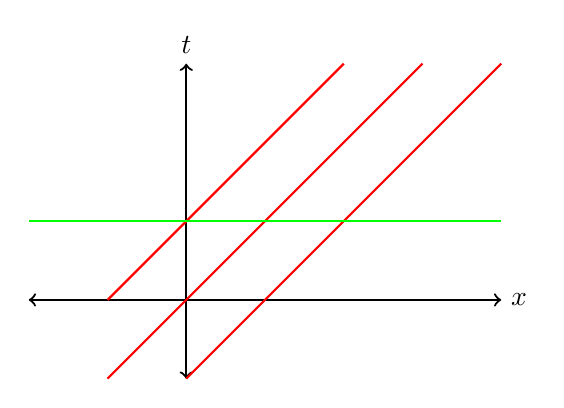
\begin{tikzpicture}[scale=1.0]
    % Draw axes
    \coordinate (nya) at (0, -1);
    \coordinate (pya) at (0, 3);
    \coordinate (nxa) at (-2, 0);
    \coordinate (pxa) at (4, 0);
    \draw [<->, thick] (nya) -- (pya);
    \draw [<->, thick] (nxa) -- (pxa);
    \node [above] (lpya) at (pya) {$t$};
    \node [right] (lpxa) at (pxa) {$x$};
    \draw [red, thick] plot [smooth, tension=1] coordinates {(-1,-1) (3,3)};
    \draw [red, thick] plot [smooth, tension=1] coordinates {(-1,0) (2,3)};
    \draw [red, thick] plot [smooth, tension=1] coordinates {(0,-1) (4,3)};
    \draw [green, thick] plot [smooth, tension=1] coordinates {(-2,1) (4,1)};
\end{tikzpicture}
\end{center}

Red lines are stationary observers, and intersection with red lines indicate simultaneous events.

\heading{Math Perspective}

Are Galilean transformations the most general transformations between inertial observers? Use axioms?

\heading{Physics Perspective}

\begin{itemize}
    \item Maxwell's equations do not transform well under Galilean transforms. Lorentz found the Lorentz transformations that allow Maxwell's equations to transform well.
    \item Michelson-Morley experiment: reveals that speed of light is invariant under the change of frame.
    \begin{itemize}
        \item $v_1 + v_2 = v_3$ This is \textbf{not} the case if $v_2 = c$
        \item $v_1 + c = c$ What why???
        \item Under the assumption that light is a wave in the ether. Results suggest that the ether is not measurable.
    \end{itemize}
\end{itemize}

\subsection{Lorentz Transformations}

Let's use light to measure objects in two frames; specifically let's determine the position using light.

\heading{Assumptions}

\begin{itemize}
    \item The speed of light is the same in any frame.
    \item Relativity Principle
    \item Bob will move at velocity $v < c$
    \begin{itemize}
        \item If an observer is moving $v > c$, their position can't be measured using light
    \end{itemize}
    \item 2d for simplicity
    \item Set $c=1$, $x=ct + x_0 = t + x_0$
\end{itemize}

\begin{center}
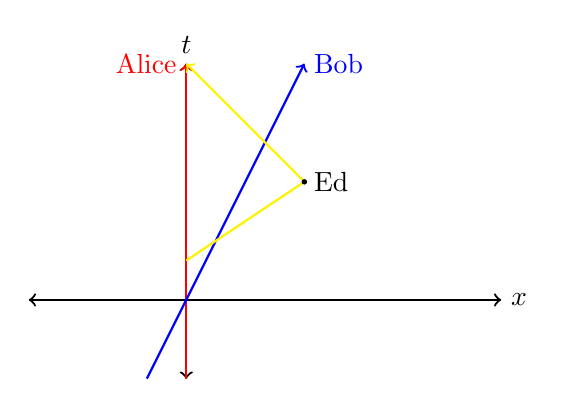
\begin{tikzpicture}[scale=1.0]
    % Draw axes
    \coordinate (nya) at (0, -1);
    \coordinate (pya) at (0, 3);
    \coordinate (nxa) at (-2, 0);
    \coordinate (pxa) at (4, 0);
    \coordinate (ed) at (1.5, 1.5);
    \node [above] (lpya) at (pya) {$t$};
    \node [right] (lpxa) at (pxa) {$x$};
    \draw [<->, thick] (nya) -- (pya);
    \draw [<->, thick] (nxa) -- (pxa);
    \draw [->, thick, red] (nya) -- (pya);
    \draw [->, thick, blue] (-0.5, -1) -- (1.5,3);
    \draw [->, thick, yellow] (0, 0.5) -- (ed) -- (pya);
    \node [left, red] (alicelabel) at (pya) {Alice};
    \node [right, blue] (boblabel) at (1.5,3) {Bob};
    \node [right] (edlabel) at (ed) {Ed};
    \fill (ed) circle[radius=1pt];
\end{tikzpicture}
\end{center}

Let's measure the coordinates of Ed in Alice's frame and Bob's frame and the map relating the times using light to measure positions.

1) Using light to measure position,

\[ x = \f{1}{2c}\br{t_2 - t_1} \]
\[ T = t_1 + \f12 \br{t_2 - t_1} = \f12 \br{t_2 + t_1} \]

\begin{center}
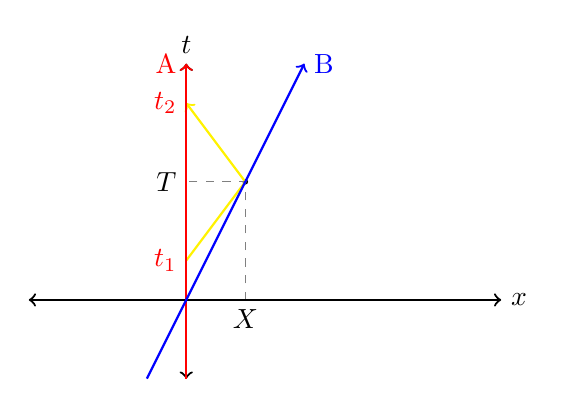
\begin{tikzpicture}[scale=1.0]
    % Draw axes
    \coordinate (nya) at (0, -1);
    \coordinate (pya) at (0, 3);
    \coordinate (nxa) at (-2, 0);
    \coordinate (pxa) at (4, 0);
    \node [above] (lpya) at (pya) {$t$};
    \node [right] (lpxa) at (pxa) {$x$};
    \coordinate (xt) at (0.75, 1.5);
    \coordinate (X) at (0.75, 0);
    \coordinate (T) at (0, 1.5);
    \coordinate (t1) at (0, 0.5);
    \coordinate (t2) at (0, 2.5);
    \node [left, red] (t1label) at (t1) {$t_1$};
    \node [left, red] (t1label) at (t2) {$t_2$};
    \node [left] (Tlabel) at (T) {$T$};
    \node [below] (Xlabel) at (X) {$X$};
    \fill (xt) circle[radius=1pt];
    \draw [->, thick, yellow] (t1) -- (xt) -- (t2);
    \draw [dashed, gray] (X) -- (xt) -- (T);
    \draw [<->, thick] (nya) -- (pya);
    \draw [<->, thick] (nxa) -- (pxa);
    \draw [->, thick, red] (nya) -- (pya);
    \draw [->, thick, blue] (-0.5, -1) -- (1.5,3);
    \node [left, red] (alicelabel) at (pya) {A};
    \node [right, blue] (boblabel) at (1.5,3) {B};
\end{tikzpicture}
\end{center}

2) Determine how the difference of times of reception and emission are related?

\[ \De t_A = ON \quad \De t_B = QP \]
\[ \f{MN}{OM} = \f{MP}{QM} \]
\[ \f{MN}{MN+\Delta t_A} = \f{MP}{MP+\Delta t_B} \]
\[ \f{\Delta t_A}{MN} = \f{\Delta t_B}{MP} \]
\[ \Delta t_A \propto \Delta t_B \]

\begin{center}
\begin{tikzpicture}[scale=1.5]
    % Draw axes
    \coordinate (nya) at (0, -1);
    \coordinate (pya) at (0, 3);
    \coordinate (nxa) at (-2, 0);
    \coordinate (pxa) at (4, 0);
    \draw [<->, thick] (nxa) -- (pxa);
    \draw [<->, thick] (nya) -- (pya);
    \node [above] (lpya) at (pya) {$t$};
    \node [right] (lpxa) at (pxa) {$x$};
    \coordinate (ai) at (nya);
    \coordinate (bi) at (-0.2, -1);
    \coordinate (af) at (pya);
    \coordinate (bf) at (1.8, 3);
    \draw [->, thick, red] (ai) -- (af);
    \draw [->, thick, blue] (bi) -- (bf);
    \node [left, red] (la) at (af) {A};
    \node [right, blue] (lb) at (bf) {B};
    \coordinate (lt0) at (intersection of nya--pya and bi--bf);
    \coordinate (lx0) at (intersection of nxa--pxa and bi--bf);

    \coordinate (M) at (lt0);
    \coordinate (O) at (0, 1.5);
    \coordinate (N) at (0, 1);
    \coordinate (P) at (intersection of O--(3,2.5) and bi--bf);
    \coordinate (Q) at (intersection of N--(3,2) and bi--bf);

    \draw [->, thick, yellow] (N) -- (Q);
    \draw [->, thick, yellow] (O) -- (P);

    \fill (lx0) circle (1pt) node[below right] {$x_0$};
    \fill (lt0) circle (1pt) node[left] {$t_0$};
    \fill (Q) circle (1pt) node[right] {$Q$};
    \fill (O) circle (1pt) node[right] {$O$};
    \fill (N) circle (1pt) node[right] {$N$};
    \fill (M) circle (1pt) node[right] {$M$};
    \fill (P) circle (1pt) node[right] {$P$};
\end{tikzpicture}
\end{center}

\[ \Delta t_A = f^{-1}(v, c, x_0, y_0) \Delta t_B \]

By translational invariance, $f$ cannot depend on $x_0$ or $t_0$. Therefore,

\[ \Delta t_A = f^{-1}(v, c) \Delta t_B \]

For convenience, we will find $f$ defined as,

\[ \Delta t_B = f(v, c) \Delta t_A \]

By similar analysis of a pair of light rays emanating from bob,

\[ \Delta \ti{t}_A = \ti{f}(v, \ti{c}) \Delta \ti{t}_B = \ti{f}(v, c) \Delta \ti{t}_B \]

This uses the assumption $\ti{c} = c$. Furthermore by the relativity principle, we must have $\ti{f} = f$. Otherwise, the two inertial frames ($A, B$) would be distinguishable through $f, \ti{f}$. In conclusion:

\[ \De t\tsb{received} = f(v,c) \De t\tsb{emitted} \]

So what is the form of $f$? Let us assume that there is a synchronization between the two frames so that calculations become easier.

\begin{center}
\begin{tikzpicture}[scale=1.5]
    % Draw axes
    \coordinate (nya) at (0, -1);
    \coordinate (pya) at (0, 3);
    \coordinate (nxa) at (-2, 0);
    \coordinate (pxa) at (4, 0);
    \draw [<->, thick] (nxa) -- (pxa);
    \draw [<->, thick] (nya) -- (pya);
    \node [above] (lpya) at (pya) {$t$};
    \node [right] (lpxa) at (pxa) {$x$};
    \coordinate (ai) at (nya);
    \coordinate (bi) at (-0.33, -1);
    \coordinate (af) at (pya);
    \coordinate (bf) at (1, 3);
    \draw [->, thick, red] (ai) -- (af);
    \draw [->, thick, blue] (bi) -- (bf);
    \node [left, red] (la) at (af) {A};
    \node [right, blue] (lb) at (bf) {B};

    \coordinate (t0) at (0, 1);
    \coordinate (tau) at (intersection of t0--(3,4) and bi--bf);
    \coordinate (tL) at ($(tau) + (0, -10)$);
    \coordinate (tT) at ($(tau) + (-10, 0)$);
    \coordinate (L) at (intersection of tau--tL and nxa--pxa);
    \coordinate (T) at (intersection of tau--tT and nya--pya);
    \coordinate (t1) at (intersection of tau--(-3,5) and ai--af);

    \draw [->, thick, yellow] (t0) -- (tau);
    \draw [->, thick, yellow] (tau) -- (t1);
    \draw [dashed, gray] (tau) -- (L);
    \draw [dashed, gray] (tau) -- (T);

    \fill (t0) circle (1pt) node[left] {$t_0$};
    \fill (tau) circle (1pt) node[right] {$\tau$};
    \fill (t1) circle (1pt) node[left] {$t_1$};
    \fill (0,0) circle (1pt) node[below right] {$S$};
    \fill (T) circle (1pt) node[left] {$T$};
    \fill (L) circle (1pt) node[below] {$L$};
\end{tikzpicture}
\end{center}

Let's define:
\begin{align*}
    \De t_A &= S \ar t_0 = t_0 \\
    \De \ti{t}_A &= S \ar t_1 = t_1 \\
    \De t_B &= S \ar \tau = \tau = \De \ti{t}_B \\
\end{align*}

Therefore $\tau = f(v,c) t_0$ with,

\[ t_1 = \De \ti{t}_A = f(v,c) \De \ti{t}_B = f^2(v,c) t_0 \]
Thus we have from radar measurements,

\[ L = \f12 c \br{t_1 - t_0} = \f12 c\br{f^2(v,c) - 1}t_0 \]
\[ T = \f12 \br{t_1 + t_0} = \f12 c\br{f^2(v,c) + 1}t_0 \]

The ratio is given by,

\[ \f{L}{T} = v = c \f{f^2(v,c) -1}{f^2(v,c) +1} \]

Inverting this expression (using $-c < v < c$) yields,

\[ f(v,c) = \br{\f{1+\f{v}{c}}{1 - \f{v}{c}}}^{1/2} \]

4) Ed's coordinate from A's and B's perspective.


\begin{center}
\begin{tikzpicture}[scale=1.5]
    % Draw axes
    \coordinate (nya) at (0, -1);
    \coordinate (pya) at (0, 3);
    \coordinate (nxa) at (-2, 0);
    \coordinate (pxa) at (4, 0);
    \draw [<->, thick] (nxa) -- (pxa);
    \draw [<->, thick] (nya) -- (pya);
    \node [above] (lpya) at (pya) {$t$};
    \node [right] (lpxa) at (pxa) {$x$};
    \coordinate (ai) at (nya);
    \coordinate (bi) at (-0.33, -1);
    \coordinate (af) at (pya);
    \coordinate (bf) at (1, 3);
    \coordinate (e) at (1, 1.5);
    \draw [->, thick, red] (ai) -- (af);
    \draw [->, thick, blue] (bi) -- (bf);
    \node [left, red] (la) at (af) {A};
    \node [right, blue] (lb) at (bf) {B};

    \coordinate (t1a) at (0, 1);
    \coordinate (t2a) at (0, 2);
    \coordinate (t1b) at (intersection of t1a--e and bi--bf);
    \coordinate (t2b) at (intersection of t2a--e and bi--bf);

    \draw [->, thick, yellow] (t1a) -- (e);
    \draw [->, thick, yellow] (e) -- (t2a);

    \fill (t1a) circle (1pt) node[left] {$T_1^A$};
    \fill (t2a) circle (1pt) node[left] {$T_2^A$};
    \fill (t1b) circle (1pt) node[right] {$T_1^B$};
    \fill (t2b) circle (1pt) node[right] {$T_2^B$};
    \fill (0,0) circle (1pt) node[below right] {$S$};
    \fill (e) circle (1pt) node[right] {$E$};
\end{tikzpicture}
\end{center}

Let $E$ be identified in two ways,
\begin{center}
\begin{tabular}{c|c}
    Alice's Perspective & $(x_A^E, t_A^E)$ \\
    \hline
    Bob's Perspective & $(x_B^E, t_B^E)$ \\
\end{tabular}
\end{center}

Therefore,
\[ x_A^E = \f12 c \br{T_2^A - T_1^A} \]
\[ t_A^E = \f12 \br{T_2^A + T_1^A} \]
\[ x_B^E = \f12 c \br{T_2^B - T_1^B} \]
\[ t_B^E = \f12 \br{T_2^B + T_1^B} \]

We know that $T_1^B = f T_1^A$ and $T_2^A = f T_2^B$ hence we can get the relation between $(x_A^E, t_A^E)$ and $(x_B^E, t_B^E)$.

\[ x_B^E = \f{1}{\sqrt{1 - \f{v^2}{c^2}}} \br{x_A^E - vt_A^E} \]
\[ t_B^E = \f{1}{\sqrt{1 - \f{v^2}{c^2}}} \br{t_A^E - \f{v}{c^2}x_A^E} \]

For convenience we can relabel,
\[ \ga =  \f{1}{\sqrt{1 - \f{v^2}{c^2}}} \]

In matrix form,
\[ \bvec{T' \\ X'} = \underbrace{\ga \bvec{1 & \f{-v}{c^2} \\ -v & 1}}_{\text{Lorentz Boost}} \bvec{T \\ X}\]

Notice in the limit that $v << c$, the Lorentz boost becomes equivalent to the Galilean boost discussed earlier.

\subsubsection{Consequences of Lorentz Transformations}

\begin{enumerate}
    \item From Alice's perspective, Bob's time axis is,
    \begin{itemize}
        \item $x^B = 0 = \ga (x_A - vt_A) \implies x = vt$
    \end{itemize}
    \item From Alice's perspective, Bob's spatial slice is,
    \begin{itemize}
        \item $T^B = 0 = \ga \br{t_A - \f{v}{c^2}} x_A \implies t = \f{v}{c^2} x$
        \item The slope of this line in Alice's perspective is the \textbf{inverse} (with $c \ar 1$) of the slope of Bob's time axis
    \end{itemize}
\end{enumerate}

Again, notice that Galilean simultaneity is recovered in the limit that $v \ar v << c$. Our new theory is still consistent with our old theories.

\end{document}